% $Id: template.tex 11 2007-04-03 22:25:53Z jpeltier $
%\documentclass{vgtc}                          % final (conference style)
%\documentclass[review]{vgtc}                 % review
%\documentclass[widereview]{vgtc}             % wide-spaced review
%\documentclass[preprint]{vgtc}               % preprint
\documentclass[electronic]{vgtc}             % electronic version

\usepackage{mathptmx}
\usepackage{graphicx}
\usepackage{times}
\usepackage{comment}
\onlineid{0}
\vgtccategory{Research}



% --------------------- Extra comment commands inserted by Jo Wood ---------------------
\usepackage[dvipsnames,usenames]{color}
\newcommand{\marrow}{\marginpar[\hfill$\longrightarrow$]{$\longleftarrow$}}
\newcommand{\joremark}[3]{\textcolor{Bittersweet}{\textsc{#1 #2:} \marrow\textsf{#3}}}
\newcommand{\jo}[2][says]{\joremark{Jo}{#1}{#2}}
% ------------------------- End of comment commands --------------------------------------------


%% In preprint mode you may define your own headline.
%\preprinttext{To appear in an IEEE VGTC sponsored conference.}

%% Paper title.

\title{Obvious: a Meta-toolkit for information visualization toolkits used in Visual Analytics}
\vgtcinsertpkg

\author{%
Thomas Baudel\thanks{e-mail:baudelth@fr.ibm.com}\\ %
  \scriptsize IBM %
\and Jean-Daniel Fekete\thanks{e-mail:Jean-Daniel.Fekete@inria.fr}\\ %
  \scriptsize INRIA %
\and Pierre-Luc Hemery\thanks{e-mail:Pierre-Luc.Hemery@inria.fr}\\ %
  \scriptsize INRIA %
\and Jo Wood\thanks{e-mail:jwo@soi.city.ac.uk}\\ %
   \scriptsize City University
}     
%% A teaser figure can be included as follows, but is not recommended since
%% the space is now taken up by a full width abstract.
%\teaser{
%  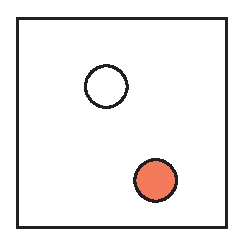
\includegraphics[width=1.5in]{sample.eps}
%  \caption{Lookit! Lookit!}
%}

%% Abstract section.
\abstract{ This article describes ``Obvious'': a meta-toolkit that
  abstracts and encapsulates information visualization toolkits
  implemented in the Java language. It intends to unify their use and
  postpone the choice of which concrete toolkit(s) to use later-on in
  the development of visual analytics applications.  We also report
  on the lessons we have learned when wrapping popular toolkits with
  Obvious, namely Prefuse, the InfoVis Toolkit, partly Improvise, JUNG
  and other data management libraries.  We show several examples on
  the uses of Obvious, showing how the different toolkits can be
  combined, for instance sharing their data models.  We also show how Weka, a
  popular machine-learning toolkits, has been wrapped with Obvious and
  can be used directly with all the other wrapped toolkits. 

  We expect Obvious to start a co-evolution process: Obvious is meant
  to evolve when more components of information visualization systems
  will become consensual. It is also designed to help information
  visualization systems adhere to the best practices to provide a
  higher level of interoperability and leverage the domain of visual
  analytics.
}



%% ACM Computing Classification System (CCS). 
%% See <http://www.acm.org/class/1998/> for details.
%% The ``\CCScat'' command takes four arguments.

\CCScatlist{ 
  \CCScat{K.6.1}{Management of Computing and Information Systems}%
{Project and People Management}{Life Cycle};
  \CCScat{K.7.m}{The Computing Profession}{Miscellaneous}{Ethics}
}

%% Copyright space is enabled by default as required by guidelines.
%% It is disabled by the 'review' option or via the following command:
% \nocopyrightspace

%%%%%%%%%%%%%%%%%%%%%%%%%%%%%%%%%%%%%%%%%%%%%%%%%%%%%%%%%%%%%%%%
%%%%%%%%%%%%%%%%%%%%%% START OF THE PAPER %%%%%%%%%%%%%%%%%%%%%%
%%%%%%%%%%%%%%%%%%%%%%%%%%%%%%%%%%%%%%%%%%%%%%%%%%%%%%%%%%%%%%%%%

\begin{document}

\firstsection{Introduction}

\maketitle

%% -*- mode: LaTeX; -*-

Over the past few years, several information visualization (InfoVis)
toolkits have flourished in various languages such as
Java~\cite{Discovery2,InfoVis, Prefuse, jung2003, Improvise},
C++~\cite{Tulip,ADVIZOR}, Flash/Flex~\cite{Axiis,flare} or
JavaScript with HTML5~\cite{thejit,Protovis} to name a few.  When starting
a visual analytics (VA) project, the choice of the toolkit is a major
initial decision and the resulting proliferation of toolkits can be confusing
for VA software developers who know that an
inappropriate choice can lead to unanticipated limitations during the
development of the application.

Historically, this proliferation of toolkits can be explained by
several factors: each created toolkit addresses a specific set of
problems, is designed with a specific application domain in mind, or
simply offers different tradeoffs.  However, it results in dispersion
in terms of capabilities since each toolkit has unique and useful
techniques for visualization and interaction.  For example, the
Prefuse~\cite{Prefuse} and JUNG~\cite{jung2003} toolkits offer several
graph layout algorithms whereas Improvise~\cite{Improvise} supports
very sophisticated coordinated views with limited graph capabilities.

The choice of an InfoVis toolkit should be made
early in the software development process because it affects not only the visualization techniques but
also the data structure to work with.  For an application dealing with
small quantities of data, copying data from one structure to another
is possible in interactive time but not for VA
applications that usually manage data sets too large to be duplicated
at all.  Therefore, most data-management and analysis will be made on
data structures compatible with the visualization and tied to the
visualization toolkit.

%\jo{changed language in the following paragraph to emphasise that this is a consequence of a lack of meta-toolkit/interface rather than advice.}

Once the choice is made, any missing components have to be added
specifically to the toolkit: if a special data manager is required
(e.g., reading a particular data format), it has to be implemented
specifically for the data structure managed by the toolkit. Any analysis
not supported by the toolkit requires the authoring or adaptation of
analytical toolkit components. Likewise, if visualization techniques
are required that are not supported by the chosen toolkit they must
be added, creating a strong dependency that usually prevents changes
of toolkit later-on in the development.

The effort required by one application to implement the missing
components cannot easily be reused in other applications that are based on another
toolkit.  Therefore, important resources are wasted for the re-implementation of
data converters, analysis modules, and visualization techniques. 

To address this proliferation problem, this article introduces
\emph{Obvious}: a meta-toolkit that abstracts and encapsulates InfoVis
toolkits implemented in the Java language as a way to unify their use
and postpone the choice of which concrete toolkit(s) to use later-on
in the development process.  Obvious is mainly targeted at VA software
developers, but also  library or toolkits developers if they want to
promote sharing of data managers, converters, or algorithms not
restricted to one toolkit.

\noindent This article presents three contributions:
\begin{enumerate}[noitemsep,topsep=0pt]
\item it describes the design and implementations of Obvious,
\item it reports some lessons learned when wrapping existing toolkits
  with Obvious, and
\item it presents rationales for the social process we started and
  want to follow for the future of Obvious.
\end{enumerate}

\noindent The main benefits offered by Obvious are:
\begin{enumerate}[noitemsep,topsep=0pt]
\item it improves the reusability of code and components;
\item it improves the interoperability of code, data models and
  visualizations;
\item it defers the choice of which concrete toolkits to use to a
  later stage of the VA development;
\item it enforces a better separation of concerns in VA
  applications so that the data models can be specified independently
  of the visualizations and views;
\item it allows toolkit and library developers to easily integrate
  their tool into the rich environment of Obvious-compatible systems;
\item it clarifies issues with notification and allows VA to scale up using a standard architecture; and
\item it specifies a set of interfaces and a stable vocabulary which
  simplifies learning.
\end{enumerate}

\begin{comment}
Obvious is implemented in a modular way with an abstract core module
and additional specific bindings, implemented for several toolkits:
the Infovis toolkit~\cite{InfoVis}, Prefuse~\cite{Prefuse},
Improvise~\cite{Improvise} and Jung~\cite{jung2003}.  These bindings
have been used to build some proof-of-concepts examples combining
different toolkits and also to create complete systems used by ongoing
research projects such as~\cite{BENZAKEN:2011:INRIA-00532552:1}.

During the development of bindings, we have seen important design
questions emerge regarding the interpretation of the reference model;
we report them here to help clarify the InfoVis reference model and
trade-offs in its implementation.

In addition, Obvious allows developers to eliminate the crucial choice
of the toolkit and to avoid rewriting existing functionalities such as
file import and export modules, as well as analytical algorithms. The
following use case shows it is now possible to combine toolkits.  For
example, they can choose a data model from JUNG toolkit for a graph,
then query it with Prefuse predicates, use a layout introduced in
Infovis toolkit to display it and still used network algorithms
introduced in JUNG.  With obvious, there are no more design restrictions
imposed by an initial choice for developer.


%\subsection{Goals and Social Process}

Obvious is not another toolkit, it is a set of interfaces that
abstract the services provided by InfoVis toolkits
implemented according to the InfoVis reference
model~\cite{ChiRefModel,ReadingsIV}.  Obvious has been specified
during a workshop gathering several major authors of
toolkits~\cite{vismaster2008}; its interfaces have reached a consensus
at the time of the workshop among the developers.  However, they do
not cover all the parts of the reference model evenly.  The data
component is much more precisely defined than the visualization and
view components. 

In the related work section, we describe several models that have been
used to standardize software 

%\subsection{Targeted uses}

A typical scenario of Obvious would be the design of
VizTree~\cite{lin01}, a VA application for monitoring
massive time-series.  VizTree encodes very long time-series of a
continuous value as a suffix tree; the details of this encoding being
beyond the scope of the paragraph scenario.  The associated tree
visualization has been implemented by specialists of data-mining and
leaves room for improvements in term of visualization and
interaction.  Using Obvious, the authors would first connect their
computed data structure to the data model of Obvious. There are two
ways of doing that: use the Obvious data-model directly or use the
native data-model implemented for mining the time-series and wrap it
with an implementation of the Obvious data-model. Both are possible
and will be chosen according to the amount of work and flexibility
offered by one option or the other. Once an Obvious data-model is
available, the authors of VisTree can start exploring which toolkit
will provide them the best support for their visualization. They can
choose among the InfoVis Toolkit, Prefuse and JUNG to visualize tree
data. Once the best one has been chosen, the interaction can be
crafted either on top of the abstraction provided by Obvious - to keep
the option of switching the final implementation - or using the native
toolkit controls to keep a tighter control of the interface. If
desired, the interface can also be improved by adding other
visualizations associated with the computation of the prefix tree or
of statistics associated with the data. If multiple-coordinated views
are required for that, Improvise visualization and views can be added
to the interface using the same data model. In that scenario, Obvious
has enabled data-mining researchers to focus on their skills and to
use state-of-the-art visualization components at a later stage of the
development of their application.

Another scenario [DDupe]

Yet another, more futuristic scenario: porting a new visualization type to multiple toolkits
or allowing cross-toolkit brushing interaction.

\end{comment}

The article is organized as follows: in section 3, after the related
work section, we describe the design of Obvious. Section 4 reports on
the wrapping of several toolkits and components with Obvious. Section
5 shows examples of Obvious in action to assess its
usefulness. Section 6 discusses the social process we have used and
how we envision the evolution of Obvious before concluding.


\section{Related Work}

Obvious is a set of interfaces and extension classes for wrapping
around existing information visualization toolkits.  It generalizes
and extends the standard architecture as defined in the Information
Visualization reference model to try to abstract all the existing
implementations.  In this section, we list some major existing
toolkits and explain what they share and how they differ.  In the
second section, we describe the most common standardization processes
for software systems.

\subsection{Visualization Toolkits}

Pretty much all existing information visualization toolkits follow the
InfoVis reference model initially specified by Ed Chi and refined by
Card, Mackinlay and Shneiderman~\cite{ChiRefModel,ReadingsIV} and has
been described as a design pattern in~\cite{DesignPatternsIV}.  The
model defines three stages: \emph{DataSet} or \emph{Data Tables},
\emph{Visualization} or \emph{Visual Structure} and \emph{View}
(Figure~\ref{fig:refmodel}).  One of its main benefits is that it
explicitly represents interaction, in contrast to older visualization
models.  Several articles have described the concrete design of an
information visualization toolkit.  We report here on the common and
the specific parts.

\begin{figure}
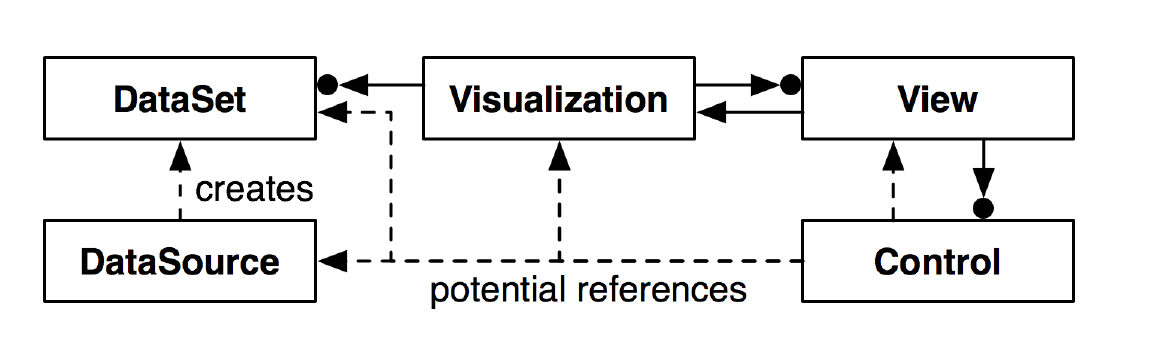
\includegraphics[width=\columnwidth]{figures/refmodpat}
\caption{The Information Visualization Reference Model~\cite{DesignPatternsIV}}
\label{fig:refmodel}
\end{figure}


The InfoVis Toolkit~\cite{InfoVis} is based on an \emph{in-memory
  database manager} where data is organized in columns --- contrary to
most persistent relational databases --- to improve the memory
footprint and allow addition of new attributes that are needed to
manage the interaction (e.g. selection or filtering) and to hold
attributes computed on demand.  The main challenge being the support
of interactive performance for rendering and dynamic queries with a
small memory footprint.  The visual structure is managed using a
\emph{monolithic} architecture~\cite{Polylithic}: each visualization
technique is implemented as a specific class
(e.g. ScatterplotVisualization, ParallelCoordinatesVisualization,
TreeVisualization) that performs the mapping between the data set and
the graphics items to render.  Finally, the view component is the same
for each of the visual structures and takes care of scrolling,
zooming, overlaying magic lenses (e.g. Fisheye or Magic Lenses).  A
\emph{notification mechanism} implements the communication between the
data tables and the visual structure: each time a data table is
modified, it notifies all the registered handlers of the details of
the modification. The interaction is managed by \emph{Interactor}
objects that are associated with the visual structures; the views are
generic and forward interaction managements to the Interactors.  One
specific feature provided by the InfoVis Toolkit is layering:
visualization can be composed on top of each others.  Composite
visualizations are useful to build complex visualization by breaking
them into simple parts. For example, node-link diagrams are split into
links managed as a layer and nodes as another.  Magic lenses and
Fisheyes are also managed as layers on top of other visualizations.

Prefuse~\cite{Prefuse} also relies on an in-memory database with
notification but implements the visual structure using an extension of
the data model (a visual table derives from a data table).  It then
transforms the data into a \emph{polylithic} graphic structures
whereas all the other toolkits use a \emph{monolithic} architecture.
In a polylithic architecture, there is only one component in charge of
all the visual structures.  A visualization object is responsible of
managing a visual structure: it contains visual tables that augment
data tables with graphic attributes (shape, color, etc.)
Visualizations are in charge of computing the layout (assigning a
position and shape to visual items), the graphic attributes and
animations.  Visualizations use a \emph{Renderer} object to actually
display visual items.  Users can control which renderer is used
depending on the visualization and the object itself.  In Prefuse,
data managers, visual managers and views are generic, offering a very
clean interface to the application programmer.  However, as noted by
Bederson at al.~\cite{Polylithic}, polylithic toolkits have a steeper
learning curve than monolithic ones because the polylithic components
do not work out of the box, they always need to be configured.  To
address this issue, Prefuse comes with code samples that simplify the
initial setup.

Building upon their experience in the Prefuse toolkit~\cite{Prefuse},
Heer et Agrawala~\cite{DesignPatternsIV} have derived software design
patterns that are common to information visualization applications and
toolkits. 

Improvise~\cite{Improvise} relies on an in-memory database with
notification that is row-oriented and its visual structures are
monolithic.  The main characteristic of Improvise lies in its
management of coordinated views.  To this aim, it relies on several
design patterns not supported by Prefuse; compared to the other
information visualization toolkits, it adds a coordination component
that is central and extends the notification mechanism implemented
by the InfoVis Toolkit or Prefuse.

Discovery~\cite{Discovery1,Discovery2,Discovery3} shares most of its
characteristics with Prefuse: it uses an in-memory, column-oriented
database and a polylithic graphic model. Its two main features are 1)
the absence of a scene graph, replaced by a dataflow pipeline made of
short operations called \emph{functors} that renders directly from the
data-model, and 2) a deferred notification strategy to allow data
editing.

%% \jo{I'm not sure I am convinced of the assertion in the following
%%   paragraph. The three toolkits above are described in some detail,
%%   not all of which is relevant to other toolkits. Perhaps we should
%%   instead abstract their distinct design characters. e.g. Row-oriented
%%   vs column oriented; in-memory vs cached database management;
%%   monolithic vs polylithic etc. The point being that while they all
%%   attempt to achieve similar general aims, their lower-level approach
%%   to doing so requires different programming approaches, hence the
%%   need for Obvious.}

Other information visualization toolkits can mostly be described using
the four toolkits above, even if they use a different programming
language.  Tulip~\cite{Tulip} is a graph-oriented toolkit programmed
in C++ that uses data tables for vertices and edges, like the InfoVis
Toolkit and Prefuse.  It implements several complex graph layout
algorithms and uses OpenGL for its rendering but the conceptual
architecture is table-based and monolithic.  Therefore, information
visualization toolkits share a global organization, they all implement
an in-memory database with two variants (row-based or column-based), a
visual structure with two variants (monolithic or polylithic) and
several specific features.  Even if some choices made by toolkits
designers were carefully decided, other were probably made without
being aware of the alternatives.  Combining the best possible features
for a next-generation toolkit might be tempting but there are still
tradeoffs that cannot be solved.  For example, the power of
coordinated and linked views offered by Improvise comes at the cost of
maintaining caches that should be flushed when the data change so
there seems to be a tradeoff there that still needs research to be
solved.

There are also lower-level toolkits that can be used to build visual
analytics applications.  Two popular families are graphics libraries
and graph libraries.

%% \jo{I'm not sure what point is being made here with the discussion of
%%   lower level visualization toolkits. Are we asserting that the
%%   standardization implied by Obvious is also appropriate for lower
%%   level approaches to VA software construction? If so, we need to
%%   identify what is lacking in an approach without Obvious as well as
%%   demonstrating (later on in the paper) that implementing the Obvious
%%   interfaces in lower level visualization environments is both
%%   practical and beneficial. An interesting test case might be
%%   \emph{Processing} (processing.org). This is, compared to the other
%%   examples cited, a very low level approach to visualization software
%%   development. However, it is designed for rapid-prototyping, and if
%%   it could be easily integrated with Obvious it might provide a nice
%%   example of how early prototypes could be transformed into more
%%   robust applications using Obvious as the bridge. I'd be happy to
%%   write some words on this if you think it fits well with the theme of
%%   the paper.}

\subsection{Graphics Libraries}

Visual analytics applications can manage their own data structure and
take care of the mapping from data to visualization on their own.  At
this point, they can use \emph{scene-graphs} or \emph{direct-graphics}
libraries.  

Scene-Graph toolkits can manage the visual structure and view as
described in the reference model.  They are focused on computer
graphics and interaction: they only deal with the visual structure and
view.  Piccolo and Jazz~\cite{Polylithic} are popular 2D scene-graph
managers that have been used to create several information
visualization applications (e.g.~\cite{SpaceTree,Geneaquilt}.) An
early version of Piccolo has also been used as graphics engine for the
Cytoscape graph visualization system~\cite{Cytoscape} but dropped for
performance reasons.

High-performance information visualization applications use
scene-graph optimization techniques to speed-up the rendering of
scenes.  Tulip~\cite{Tulip} and Gephi~\cite{Gephi} maintain a spatial
indexing structure to avoid rendering objects that are not visible.

Although scene-graph technologies are mature and used in a wide
variety of graphics applications such as games, virtual-reality
applications and scientific visualization systems, they are not always
adequate for information visualization systems because they require
the explicit specification of geometry and graphic attributes for each
displayed objects.  Very often, information visualization can quickly
compute graphic attributes and even geometry from data attributes.
For example, the position of an item using a scatterplot visualization
is computed using a simple affine transformation the data attributes
using for the X and Y dimensions.  There is no need to store the
computed values when computing them on the fly is very cheap.  The
same is true for color etc.  Copying and storing this information is
costly in terms of time and memory.

Direct-graphics libraries such as \emph{Processing} or \emph{OpenGL}
can also be used to implement the visualization technique while
drawing for rapid prototyping or high-performance reasons.

[Add a section on Processing]

Still, when separating the data-model from the visual model,
scene-graph managers offer more flexibility than information
visualization systems for complex graphics and sophisticated
interaction.  This is why several information visualization systems
still use them.

% say something about the fact that scene-graph toolkits are
% classically for 3D scenes.

\subsection{Graph Libraries}

While most table-based visualization toolkits rely on an in-memory
database, several graph-based visualization systems manage their
data-structures using a model inspired from graph-theory where
topology is the main focus and data associated with graph entities is
less important.  This is the case for the JUNG library~\cite{jung2003}
or the Boost Graph Library (BGL)~\cite{BGL}, as well as for the graph
library used by Cytoscape~\cite{Cytoscape}.

These libraries support graphs as set of vertices and edges (the
topological entities) that can be associated with arbitrary data.
This data is just stored by the graph entities as a convenience for
the application: the library does not implement any integrity check
between data and graph entities.  In contrast, the InfoVis Toolkit,
Prefuse and Tulip maintain a close consistency between graphs and data
tables: removing a data table entry associated with a graph entity
(vertex or edge) also removes the entity from the graph structure.

Thus, there is no clear consensus on how a graph data structure should
be managed internally; the design choices are quite different
depending on the communities such as graph theory, information
visualization, database and semantic web.


\subsection{Standardization Processes}

Standardization is a well established habit in the software community;
several standardization models have been used in the past and these
models tend to evolve due to the growing pace of software development
taking place nowadays.

Standards have been specified by national and international
organization such as the International Organization for
Standardization (e.g. ISO, ASCII), non-profit organizations (e.g. the
Unicode Consortium or OMG), consortia of public or private
organizations (e.g. the World Wide Web Consortium (W3C)). Closer to
the information visualization community, ``The Open Geospatial
Consortium (OGC)\footnote{\url{http://www.opengeospatial.org}} is an
international industry consortium of 423 companies, government
agencies and universities participating in a consensus process to
develop publicly available interface standards.''

\jdf{More to come..}


\section{Design Overview}



Beyond proposing a unifying design, perhaps the most novel approach of Obvious is the \emph{process} carried to obtain this design.
The project started through a sequence of Information Visualization Infrastructure workshops~\cite{visinfrastructure1,visinfrastructure2,vismaster2008},
during which consensus was reached that:
\begin{enumerate}
\item many common traits were shared among toolkits, often in slightly incompatible ways.
\item much mundane work was needlessly repeated accross toolkits.
\item creating a unified toolkit from scratch was out of reach due to varying needs and design tradeoffs
\end{enumerate}
Based on those observations, consensus was reached to try the new approach of defining a "meta-toolkit" that would allow at first sharing and implementing
cross-compatible services (such as data readers), then design and implement, one by one, the components on which common consensus could be reached 
for a unified design.

For this reason, Obvious is organized according to the Information Visualization Reference Model in three main packages: data, visualisation and view. Additionally, it provides utility classes in the util package. Next, efforts were focused on designing a consensual data model. To this day, the data model is the most elaborated and successful part of the framework. Subsequent efforts shall focus on the next modules of the Visualization Reference Model, even though simple stubs for these packages have already been successfully designed.

Resting on these fundation modules (data, visualisation, view), some actual service packages have been developed, such as data readers, or shall be developed, such as dimension to scalar functors, to provide immediate utility to both the Obvious users and the toolkit designers.

\jo{It seems to me that there were two categories of contributors to the consensus. Firstly there were the developers of existing comparatively generic vis toolkits (InfoVis Toolkit, Prefuse, Improvise). While they had different approaches to their architecture (as detailed in the previous section), they are all relatively application-agnostic. This has understandably had the main influence on the design of Obvious since they are sufficiently generic to offer wide applicability to other toolkits.  Then there developers who worked with specific types of data or application (Jung, Cytoscape, LandSerf~\cite{wood_terrain_2008}, Mondrian). These data/applications have particular character that shaped the design of the Obvious interface (e.g. need for robust graph handling; need for geospatial raster handling; statistical graphics). Sometimes these application areas fit well with the initial Obvious interface (e.g. JUNG graphs), but some others were a little more problematic (e.g. large geospatial rasters can be modelled as tables, but not particularly efficiently. This raises the design question as to what extent Obvious should accommodate these application areas and to what extent should they adapt their internal architectures to accommodate a common Obvious framework? I think this would lead nicely into the next section that provides details on the Obvious data model.}




\section{Data Model}

This section describes the data model used in Obvious to represent and
manipulate data structures.  This model has been specified for the
most part during the 2008 workshop~\cite{vismaster2008} as consensus
has emerged, tediously but rapidly on its central and annex features.

\begin{figure}[!ht]
\centering
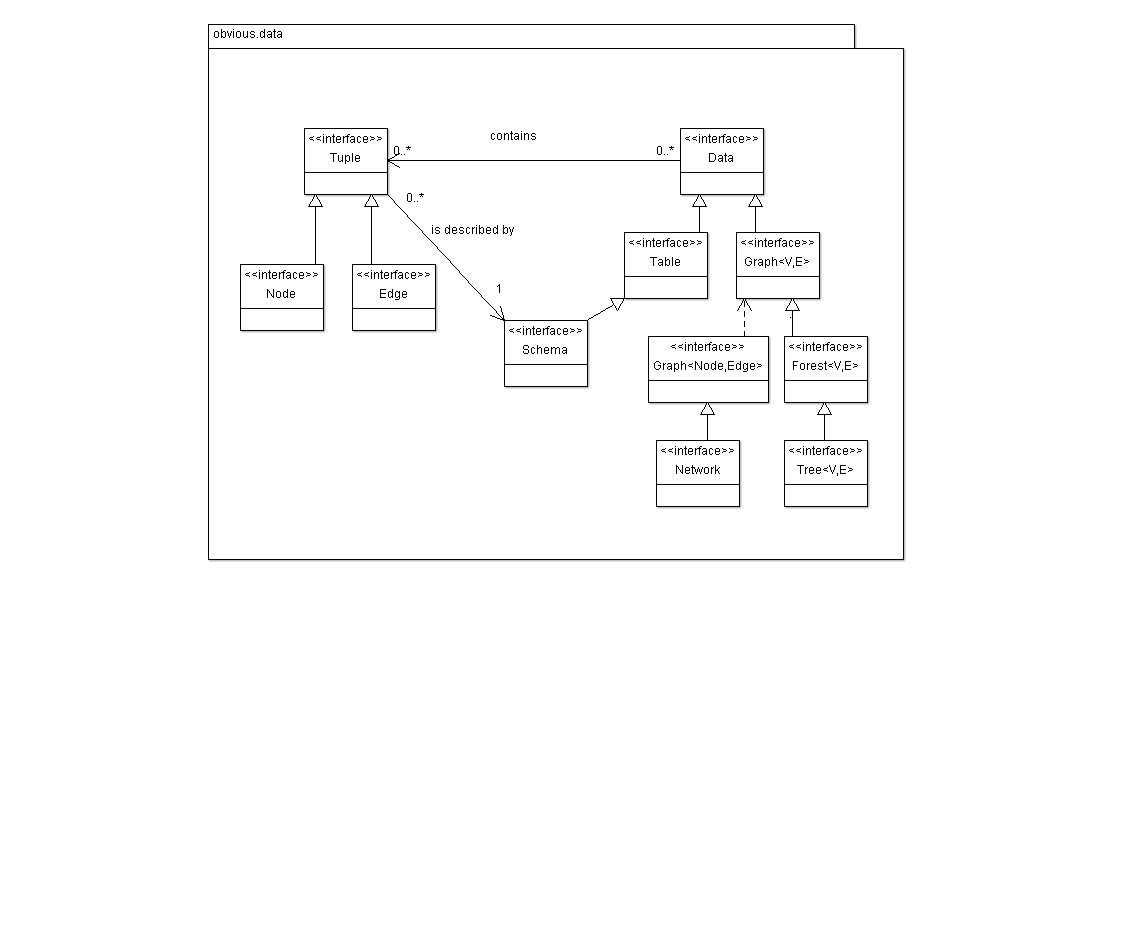
\includegraphics[width=0.7\columnwidth]{figures/obviousdataclass}
\caption{Class diagram of the Obvious data model}
\label{fig:datamodel}
\end{figure}

The Obvious data model (Figure~\ref{fig:datamodel}) is centered on the
proxy tuple design pattern exposed in \cite{DesignPatternsIV}. Obvious
adopts this design pattern to offer high extensibility and good
usability.  Among all the patterns introduced
in \cite{DesignPatternsIV}, the proxy tuple pattern enables both as it
encompasses graphs in an object-oriented manner --- many developers
are used to manipulation of \emph{object oriented graphs} ---- and as
it unifies the data model around the same standard structure (tuples
and tables). In our data model, tuples are standards elements of all
structures: tables are composed of tuples and graphs/trees are
implemented as networks, i.e., graphs built around two tables one for
the nodes and the other for the edges.

This model is instantiated via factories that allow cross-toolkit
interoperable data structure instantiation. With those factories, it
is possible to instantiate tables and networks from a schema or from
an existing object from a targeted Obvious implementation (e.g. a
Prefuse table or a JUNG graph). This also provides the possibility
to use parameters to provide more arguments used in targeted
toolkits. For example, in the Prefuse implementation of Obvious,
parameters are used to specify the source and target node columns for
a graph in an edge table.

In addition to data access, our data model provides 3 optional,
interoperable, features: \emph{introspection}, \emph{batch editing},
and \emph{notification}. Those features are not found in all target
toolkit implementations and, thus, sometimes had to be emulated.
 
\subsubsection{Introspection}

Introspection means the capability of a program to inspect its own
content. In the context of the data model it means mostly that objects
expose their own schema explicitly and allow manipulating it as a
full-fledged object.  As an improvement over \cite{DesignPatternsIV},
our data model uses a meta-circular schema design (the schema is
itself a table) instead of a column object, that does not exist in
Obvious.  Schemas have been introduced because they are an efficient
an elegant mean to gather all \emph{meta-data} for the columns of a
table in one unique structure, allowing easy table and network
instantiations with a factory.  The main use of introspection in a
toolkit, though, is to enable generic implementation of a variety of
side services as varied as generic persistence, undo/redo, and
universal object editors.

\subsubsection{Batch Editing}

Batch editing means that one or many cells in a data model may be
edited at the same time.  This happens when the toolkit manages
analytical columns (e.g. computing the centrality of each vertex in a
network), with selection and dynamic queries if their effect is
reported to a data column or simply if a user wants to change values
interactively, either in the data table or through a visualization by
direct manipulation~\cite{Discovery3}.

\subsubsection{Notification}

All the popular InfoVis toolkits
(e.g. \cite{Prefuse, InfoVis, jung2003, Discovery1}) implement
notification using the ``Observer'' pattern from~\cite{DesignPatterns}
to propagate information about changes affecting the data model.  This
pattern specifies two roles: Observable and Observer; in our case,
data models are Observables meaning that they allow Observers to
register and be notified when they are changed.  During the design of
Obvious, we realized there were some variants in the way toolkits
implemented this pattern.  This is why the notification system
introduced in Obvious is designed to support a wide variety of
notification models, even those not currently implemented in current
toolkits but that will be required to scale.  The notification system
in Obvious is also based on the Observer design pattern with
extensions to supports transaction and batch techniques usually found
in database system.

%\subsubsection{Combining Notification and batch editing}
\label{sub:combiningnotif}

Combining Notification and batch editing raises a challenge: since one
operation can affect a large amount of data, a flow of notifications
concerning the same action will be generated.  If each change is
managed in isolation, the application can spend a large amount of time
updating visual structures, e.g. recomputing a layout for each
modified item.  This typically leads to the application being
unresponsive for a long time.

\begin{figure}
  \centering
	\begin{sequencediagram}
        \global\def\unitfactor{0.5}
		\newthread{table}{Table}{Table}
		\newinst[2]{lstnr}{Listener}{Listener}
			\begin{callself}{table}{addRow(Tuple tuple)}{}
			\end{callself}
			\begin{call}{table}{tableChanged(...)}{lstnr}{Change propagated}
			\end{call}
			\begin{call}{table}{beginEdit(int mode)}{lstnr}{}
			\end{call}
			\begin{callself}{table}{addRow(Tuple tuple)}{}
			\end{callself}
			\begin{call}{table}{tableChanged(...)}{lstnr}{Custom strategy}
			\end{call}
			\begin{callself}{table}{addRow(Tuple tuple)}{}
			\end{callself}
			\begin{call}{table}{tableChanged(...)}{lstnr}{Custom strategy}
			\end{call}
			\begin{call}{table}{endEdit(int mode)}{lstnr}{}
			\end{call}
	\end{sequencediagram}
	\caption{Sequence diagram for the notification system}
	\label{fig:notification}
\end{figure}

\begin{comment}
\begin{figure}[!ht]
  \centering
  
\includegraphics[width=.5\columnwidth]{figures/notification}

  \caption{Sequence diagram for the notification system}
  \label{fig:notification}
\end{figure}
\end{comment}

Thus, Obvious introduces a method to control the management of batch
notifications: the \emph{beginEdit/endEdit} mechanism.
Figure~\ref{fig:notification} shows the sequence diagrams of the
notification manager.  Each time a data table is changed, the change
is transmitted to the Observer with a call to the \emph{tableChanged}
method.  This method takes several arguments describing the current
event (affected Table, rows, columns, and operation type): this is the
typical Observer pattern.

When the \emph{beginEdit} method is called on an Obvious data table,
the Observer's \emph{beginEdit} method is called to start a batch
editing transaction.  Different strategies can be applied by the
observer.  A \emph{mode} parameter allows the observer to select a
specific strategy depending on the type of transaction (atomic or
batched).  Note that the observer will still receive a tableChanged
call for each tuple modified.  The observer is in charge of
implementing a strategy to optimize atomic/batch edition.  If it does
not, the standard behavior will happen and batch editing will flood
the observer --- which is acceptable in some cases.  The following
strategies have already been developed in one or more Obvious
implementations:

\paragraph{Lazy strategy} after a beginEdit, the observer ignores all the
  tableChanged calls until the endEdit method is called; then, the
  observer's actions are performed e.g. a layout is recomputed.

\paragraph{Batch strategy} after beginEdit, the observer buffers the
  information sent by tableChanged.  When endEdit is called, the
  actions are performed on each of the buffered items.  Note that 
  buffering can be complicated when items are created, deleted or
  changed many times.  The burden is left to the observer since this
  management can be heavily optimized depending on the action to
  perform.

\paragraph{Transaction strategy} after beginEdit, the observer buffers the
  information sent by tableChanged.  When endEdit is called, it first
  checks structural invariants (for example, no null value for a
  specific field) before performing its actions on the modified items.

The \emph{beginEdit/endEdit} mechanism has been added to support batch
editing and also database transactions.  When the data model
implementation relies on a transactional database, atomic and batch
transactions will occur and notifications (e.g. implemented as
database triggers) will arrive in batches.  The semantic of Obvious
notification handles this case correctly but the observer should be
aware that the tableChanged method can be called much later than when
the table is actually changed.  This is the case for database atomic
transactions: the actual notification is propagated after the end of
the transaction when the database engine has done all the integrity
checks.

In practice, the three strategies we have described have been
sufficient so far to handle all the cases required inside toolkits.
The impact on performance can be substantial, in particular to manage
dynamic data, a very standard situation in VA
applications that has not been well addressed in InfoVis so far.


\subsubsection{Other services}

To leverage our core implementation and offer some immediately useful
services to Obvious users, we have defined a utility package
``obviousx'', named in the same way as the Java extension package
``javax''.  This package provides different kinds of utility classes
for the Obvious data model.  First, we have defined reader and writer
interfaces allowing the creation of gateways between the Obvious data
model and common data formats such as CSV and GraphML.  It provides
software developers a standard way to import and export data in
Obvious whatever the underlying implementation of the data model
is.  In addition, for data providers, it simplifies their work because
they only have to develop one reader and one writer to be compatible
with a large number of toolkits.

With the same logic, obviousx provides compatibility classes to use
with standard Java components such as a Java Table Model that allows
the creation of a JTable from an Obvious table.  Finally, obviousx
also provides wrappers to \emph{map} obvious data structures into
common existing data structures (e.g. for Prefuse, IVTK, and Jung) to
share data structures when using more than one data model.



\section{Visualization and View models}

\label{sec:viewvis}
Unlike the data model, no consensus emerged concerning the
Visualization and View models during the
workshop~\cite{vismaster2008}; the main reason being the different
approaches chosen among toolkits.  One important issue is the
monolithic vs. polylithic approach. Another one is related to tables
vs. objects: some toolkits keep the visualization data in tables
(e.g. Prefuse, the InfoVis Toolkit and Tulip) whereas others create
objects for displaying (e.g. Improvise, Cytoscape) or nothing at all
when there is a pipeline as in Discovery.  So, more work is needed to
design the abstractions required to wrap the different
implementations.  Further discussions and workshops will address the
problem.

Still, Obvious provides a solution: it wraps visualizations into a
black box with a small set of methods and, for the creation of these
visualizations, it relies on a \emph{Factory} design
pattern~\cite{DesignPatterns}.  For example, creating a scatter-plot
visualization from a data table requires the following lines:
\lstset{frame=single,columns=flexible,numbers=left,numberstyle=\tiny,basicstyle=\small,language=Java,caption={Creating a
    visualization using a Factory},label=factory1}
\begin{lstlisting}
Map params = new HashMap();
params.put("x", "id");
params.put("y", "age");
Visualization vis = VisualizationFactory.getInstance()
    .createVisualization(table, null, "scatterplot", params);
\end{lstlisting}
The variable ``param'' contains parameters to configure the
visualization, here to specify which attribute will be used for the X
and Y axes.

With this mechanism, it looks as if Obvious were a monolithic toolkit
but the actual implementation of the Obvious wrapper for a polylithic
toolkit can easily translate a monolithic specification into a
dedicated configuration for the underlying polylithic component.  The
code above will work for the Prefuse toolkit and return a polylithic
component wrapped as an Obvious visualization and configured as a
scatter-plot visualization.

If a developer needs a visualization component that does not exist in
the default implementation (e.g. an InfoVis Toolkit time-series with a
Prefuse-wrapped data table), the visualization can be created directly
from a specified factory or from the Obvious class
(e.g. \lstinline!new IvtkTimeSeriesVis(table, null, "timeseries", params)!).

%% \jo{Can we sure about the last sentence above?. The discussion of
%%   Prefuse in 6.1 is an example of this, but requires the user of
%%   Prefuse to develop new visualization components and wrap them in
%%   Obvious. This seems like an 'extra cost of development' to me.}
%% \pierreluc{Wrap them in Obvious is pretty easy (about ten lines of
%%   code). So yes, there is a tiny extra cost of development.}

An Obvious visualization works with any Obvious data model.  The data
model will be either wrapped to become compatible with the native
model if the underlying implementations are different or unwrapped
when the visualization and the data model are from the same
implementation (e.g. Prefuse).

This mechanism avoids copying data from one structure to another,
which is a crucial point for visual analytics.  Alternatively, Obvious
also provides a default mechanism to quickly copy and synchronize data
models when no wrapper has been defined for a specific toolkit.
Current wrappers are lightweight, adding very little overhead to the
system.

At this point, the application developer can choose one of the
existing visualizations from one of the wrapped toolkits or decide to
create a new one which can derive from one of the wrapped toolkits or
be implemented from scratch.  Obvious substantially increases the
number of possible visualizations and toolkits to use and does not
limit the developer in any way at this stage.

A \emph{View} is simply specified as a black box implementing a
simplified version of the camera pattern introduced in
\cite{DesignPatternsIV} to support standard operations such as zoom
and pan.  Like the visualization interface, future workshops should
enrich it when a more consensuses are reached.

%\jo{The assertion made in this section suggests that the mono/poly-lithic approaches that vary between existing toolkits have less of an impact on data models than on view models. We should probably make some reference to this distinction in Section 2 so that it does not look like we simply ran out of time in the workshop to consider standardization of view models.}


\section{Implementations}

This section points the lessons learned during implementations binding
Obvious interfaces to wrappers around concrete toolkits.  Each toolkit
has its own design choices that are discussed in articles but some of
the implications came to light when implementing the bindings, for
example differences of interpretations of design patterns.  We briefly
describe the most important lessons here.

\subsection{Prefuse}

Prefuse was the first binding implemented because its architecture is,
by design, very close to Obvious.  The binding implements all the
abstractions described in the core Obvious interfaces for all data
models, visualizations and views.

For the visualization, Prefuse is currently the only polylithic
Information Visualization toolkit with an binding for Obvious.  As
explained in~\ref{sec:viewvis}, Obvious does not offer a visualization
abstraction for polylithic components.  Thus, Obvious provides
components pre-configured for well know visualization techniques such
as scatter-plots or force directed graphs.  Currently, if a software
developer wants visualize an Obvious table using a Prefuse
visualization not offered in the Obvious visualization factory, the
only requirement is to convert the data model to a Prefuse data table
using an obviousx component.  

%% [jdf] we never mentioned predicates
%% Prefuse have also been used to implement and test predicates for all
%% the implementations of the Obvious data model. Since an Obvious tuple
%% can easily be wrapped into a Prefuse one, the first Obvious predicate
%% implementation is based on Prefuse predicate engine and its syntax.

Several interfaces defined by Obvious are based on a Prefuse concrete
class.  Therefore, Prefuse was used as a complete implementation of
Obvious to check its model and syntax.

%% This demonstrates that creating an implementation of Obvious allows
%% other implementations to benefit of new features. It is one of the
%% main goal of Obvious: binding toolkits to extend their capabilities.

\subsection{InfoVis Toolkit}

Since the Infovis Toolkit is monolithic and follows the reference
Information Visualization model, its Obvious binding realizes all the
interfaces for the data model, visualization and view introduced in
Obvious.

Since the InfoVis Toolkit has monolithic visualizations, providing
them simply consisted in wrapping them in an Obvious visualization
class and implementing a factory to create them by name.

However, the data model of the InfoVis Toolkit differs from Obvious
for trees and networks: in the Infovis Toolkit, the Graph interface is
not a super-interface of the Tree interface.  In addition, some data
model classes are more specialized in the Infovis Toolkit than in
Obvious. For example, tables can be described as static tables or
dynamic tables.  The binding was therefore complicated by these
mismatches that needed more code and a more complicated development
than for Prefuse.

Nevertheless, the InfoVis Toolkit binding is operational and
reliable.

\subsection{Improvise}

Currently, the Obvious implementation based on Improvise only
implements the data model part for tables.  Even if Improvise is a
monolithic toolkit, Obvious cannot directly bind Improvise
visualization components because the toolkit does not expose its
visualization pipeline publicly: Improvise components are intended to
be complete black boxes.  Addressing this problem would require some
changes inside the current version of Improvise. In addition,
Improvise does not support well dynamic data, which is a functionality
intended to be in every obvious implementation.

Currently, Improvise can use a data table from an Obvious data table
but the rest of the Improvise pipeline is hidden from
Obvious. Providing a complete binding for Improvise in Obvious would
require some changes in Improvise.

\subsection{JDBC}

JDBC is the standard Java interface to standard SQL databases.  We
wrapped JDBC in an Obvious data table to prove that Obvious can
support a large variety of data model, not only models coming from
information visualization toolkits.  JDBC was chosen because databases
are frequently used as data sources for applications and since JDBC
provides additional features not available in the toolkits data tables
such as atomic and batched transactions.  We used it to test the
notification model introduced formerly.  As expected, this
implementation only supports the data model of Obvious.

Concretely, this implementation translates obvious methods into SQL
queries.  For example, the data table ``get'' methods are implemented
as SELECT queries, the ``set'' methods as UPDATE queries, the ``add''
methods as INSERT queries, and the ``remove'' methods as DELETE
queries.  Queries are written in standard SQL and several applications
have been written to work with different DBMS such as MySQL and
Oracle.  In addition, for the notification system, table listeners
compatible with transaction and batch strategies presented in
\ref{sub:combiningnotif} have been developed and help validate the
Obvious notification model.

\subsection{JUNG}

JUNG is a graph library in Java that mainly manages the graph topology
but associates arbitrary attributes with vertices and edges.
Concretely, this implementation realizes all interfaces defined in
Obvious, except for tables and schemas since these notions do not
exist in JUNG.  Schemas are mandatory in Obvious, so this
implementation uses a default schema implementation from the obvious
core package.  The network structure of Obvious is similar to JUNG's
graph; therefore, the data model of JUNG was easy to wrap as an
Obvious Network.  Concerning the visualizations and views, JUNG
provides monolithic visualizations.  The Obvious implementation simply
binds existing JUNG visualization components to Obvious visualizations.

This implementation was the easiest to create since Obvious and JUNG
share common hypotheses: for their data model (Obvious network and
JUNG graph are equivalent) and JUNG and Obvious are both compatible
with the monolithic approach.  


\subsection{Units tests}
\label{sub:unittests}

Obvious is specified using Java interfaces and some comments in the
implementation files but without any formal specification of the
precise behavior of the defined interfaces.  To very that all the
implementations behave consistently, we have implemented \emph{Unit
  Tests}: a suite of classes aimed at testing all the methods of all
the classes.

Currently, the tests are only defined on the data model of Obvious.
The level of specification of Obvious visualizations and views is not
sufficient to perform useful tests.

Unit tests need an implementation to work, they cannot test abstract
classes or interfaces.  Due to the similarities of Obvious and
Prefuse, the Prefuse binding has been used to set up the unit tests
for the data model of Obvious.  They have then been moved to the core
Obvious module to be usable by all the bindings.  Unit tests allow
authors of Obvious bindings to automatically test whether their
implementation behaves in conformance with the intended semantics of
Obvious.  Also, authors are able to extend these existing tests to
perform more advanced ones for their binding.

Concretely, unit tests have been defined with JUnit~\cite{JUnit} for
the following interfaces: Schema (14 tests), Table (11 tests), Network
(13 tests) and Tree (8 tests); all part of the Obvious core package.
These tests have been systematically run for each new Obvious data
model development: all presented implementations successfully passed
those tests.


\subsection{Lessons learned}

+++ revise

We have learned several lessons during the development of Obvious
bindings:
%implementations: mainly concerning lack of precision in the
%Information Visualization reference model. We can list the following
%lessons:

\begin{itemize}
\item the need for a specification of a clear semantic for the
  notifications; the notification model can support simple models and
  more advanced ones (with batches and transactions for example)
\item the need for support for a polylithic approach to define an
  abstraction model for visualizations
\item the more abstractions defined the more unit tests we can define
  to validate new implementations
\item toolkits need to adopt patterns close to Obvious ones in order
  to enhance code quality of the implementations and to facilitate the
  sharing of functionalities among existing toolkits
\end{itemize}

\jo{The last itemized point above seems like an important one, and one we should revisit in the conclusion. It exposes the issue of the degree to which existing toolkits need to adapt to allow interoperability through Obvious. It is good that we are honest about this, but it does seem to be a significant weakness with the approach, especially if we wish to support VA that use data structures that don't fit well into those modelled in Obvious (e.g. geospatial Rasters, fuzzy sets).}





\section{Evaluation}

Formally evaluating the effectiveness of a meta-toolkit for visual analytics is complex. Arguably the most convincing method would require two groups of programmers of equivalent skills to implement the same set of visual analytics programs with and without Obvious. Then, a judgment could be made from the time spent and the quality of the results. This methodology has been used to assess the InfoVis Toolkit [4] with students but is impractical for real Visual Analytics applications that are more complex and would not fit the scope of student projects.

Another method, used to validate Prefuse [3] would be to re-implement complex Visual Analytics applications using Obvious and assess the results, again in term of time and quality. This is what we have done and we report on our results here.

\subsection{Coding applications with Obvious}

This section shows how Obvious can implement common applications in information visualization such as the creation of a scatterplot or of a graph visualization. These examples explain how to combine obvious component to build an application, how to create data structure and spot patterns to use. The first usecase concerns the coding of a graph visualization with Obvious InfoVis Toolkit implementation and the second one based on the coding of a scatterplot by combining component from different Obvious implementations.

For both examples and in fact every creation of an Obvious application, developpers have to follow the same steps:

\begin{itemize}
 \item creation of an Obvious data structure, three ways exist:
 \begin{enumerate}
  \item wrapping an existing data structure from a targeted toolkit as shown in first example
  \item using an Obvious reader to load an Obvious structure from a well known file format (CSV, GraphML...) as shown in the second example
  \item using Obvious methods to directly manipulate the data structure (addRow, addNode, addEdge...), this is not shown in both examples 
 \end{enumerate}
 \item creation of an Obvious visualization with the created data structure and a map of parameters
 \begin{enumerate}
  \item as shown in the second example, it is possible to combine data structure from one Obvious implementation with visualization from another Obvious implementation
  \item the map parameter allows developpers to customize the Obvious monolithic component (in the second example, the map indicates columns used for X and Y axis of the scatterplot)
 \end{enumerate}
 \item creation of an Obvious view with the created visualization
\end{itemize} 

\lstset{frame=single,columns=flexible,numbers=left,numberstyle=\tiny,basicstyle=\small,language=Java,caption={Visualizing a graph with Obvious},label=codeSample1}
\begin{lstlisting}
// Creates the graph structure. First, set the factory to use (ivtk).
// Then load the native data structure, and get a factory instance.
// Finally, call the convenient getter of the factory.
System.setProperty("obvious.DataFactory",
    "obvious.ivtk.data.IvtkDataFactory");
infovis.Graph g = Algorithms.getGridGraph(10, 10);
DataFactory factory = DataFactory.getInstance()
Network network = factory.createGraph(g);

// Creates the associated visualization using the
// factory for visualization. No predicate and extra
// parameters are given to the constructor.
Visualization vis = new IvtkVisualizationFactory()
    .createVisualization(network, null, "network", null);

// Creates the view. No predicates and extra parameters are given to
// the constructor.
View view = new IvtkObviousView(vis, null, "graphview", null);
// Standard Java window creation
JFrame frame = new JFrame();
JScrollPane panel = new JScrollPane(view.getViewJComponent());
frame.add(panel);
frame.pack();
frame.setVisible(true);
\end{lstlisting}

\lstset{frame=single,columns=flexible,numbers=left,numberstyle=\tiny,basicstyle=\small,language=Java,caption={Combining different Obvious implementations to display a scatterplot},label=codeSample2}
\begin{lstlisting}
// Defining the data factory to use,
// obvious-prefuse will be used for the data structures.
System.setProperty("obvious.DataFactory",
    "obvious.prefuse.PrefuseDataFactory");
// Creating an Obvious CSV reader and loading an
// Obvious table
CSVImport csv = new CSVImport(new File("example.csv"), ',');
Table table = csv.loadTable();

// Creating the parameter map for the monolithic object.
Map<String, Object> param = new HashMap<String, Object>();
param.put(IvtkScatterPlotVis.X_AXIS, "id"); // xfield
param.put(IvtkScatterPlotVis.Y_AXIS, "age"); // yfield

// Creating the visualization then the view. No predicates are given to
// the constructor.
Visualization vis = new IvtkScatterPlotVis(table, null, "plot", param);

View view = new IvtkObviousView(vis,  null, "plot", null);
// Standard Java window creation
...
\end{lstlisting}

\subsection{Example using Weka}

Weka \cite{Weka} is a suite of machine learning software widely used to design applications particularly for visual analytics \pierreluc{I should put a reference here to justify this affirmation. Can you suggest one?}. Thus, Obvious in its obviousx package supports mechanisms to build Instances (main data structure of Weka) from Obvious Table. Several methods exist to link an Obvious structure with a Weka one:

\begin{itemize}
\item an Obvious table can be loaded into a Weka Instances. Since "Instances" is a data structure specially optimized for fast processing with clustering and machine learning algorithms, with this approach the developer benefits from Weka optimizations in terms of execution time.
\item an Obvious table can wrap a Weka Instances: Obvious tables translates its methods to Weka ones. With this approach, data are not duplicated in memory.
\end{itemize}

Both methods are equivalent in terms of lines of code and can be completed with the same machine learning algorithms from Weka. For instance, to wrap an existing table into a weka Instances, developpers simply need to add the following line to the code sample \ref{codeSample2} :

\lstset{frame=single,columns=flexible,numbers=left,numberstyle=\tiny,basicstyle=\small,language=Java,caption={Wrapping an Obvious Table into Weka Instances},label=wekaExample}
\begin{lstlisting}
Instances inst = new ObviousWekaInstances(table, "Instances");
\end{lstlisting}

To wrap the Obvious structure, the constructor simply needs as argument the Obvious table and a name for the weka Instances. Then, developpers can apply to this new Instances all machine learning algorithms defined in Weka. Creating this wrapper takes less than a week for one developper knowing well Obvious but discovering Weka.

This example demonstrates an important gain of Obvious: when a toolkit adopts Obvious it can immediately benefit from existing wrappers to complementaries functionalities. Thus, with the obviousx.weka package, all Obvious implementations can now provide advanced machine learning capabilities to their users.

\subsection{EdiDuplicate (a DDupe-Like application)}

INRIA maintains a database for the publication of its member. Researchers regularly fill this database, called HALINRIA, with their new publications. However, mistakes often appears during this process: duplicated authors, institutions or papers. That is why Obvious has been used to create a DDupe like application to detect duplicated authors in the database.

DDupe is a software initially written in .NET dedicated to detect and merge duplicated nodes (often modeling people)  in (social) network to facilitate data analysis. It uses similarity metric to compare each pair  of authors and class results in descending order of similarity. In addition, DDupe allows the user to see the neighbourhood of the pair of nodes before merging them, in order to check if common nodes exist among their neighbors and then to confirm metric results.

\begin{figure}[!h]
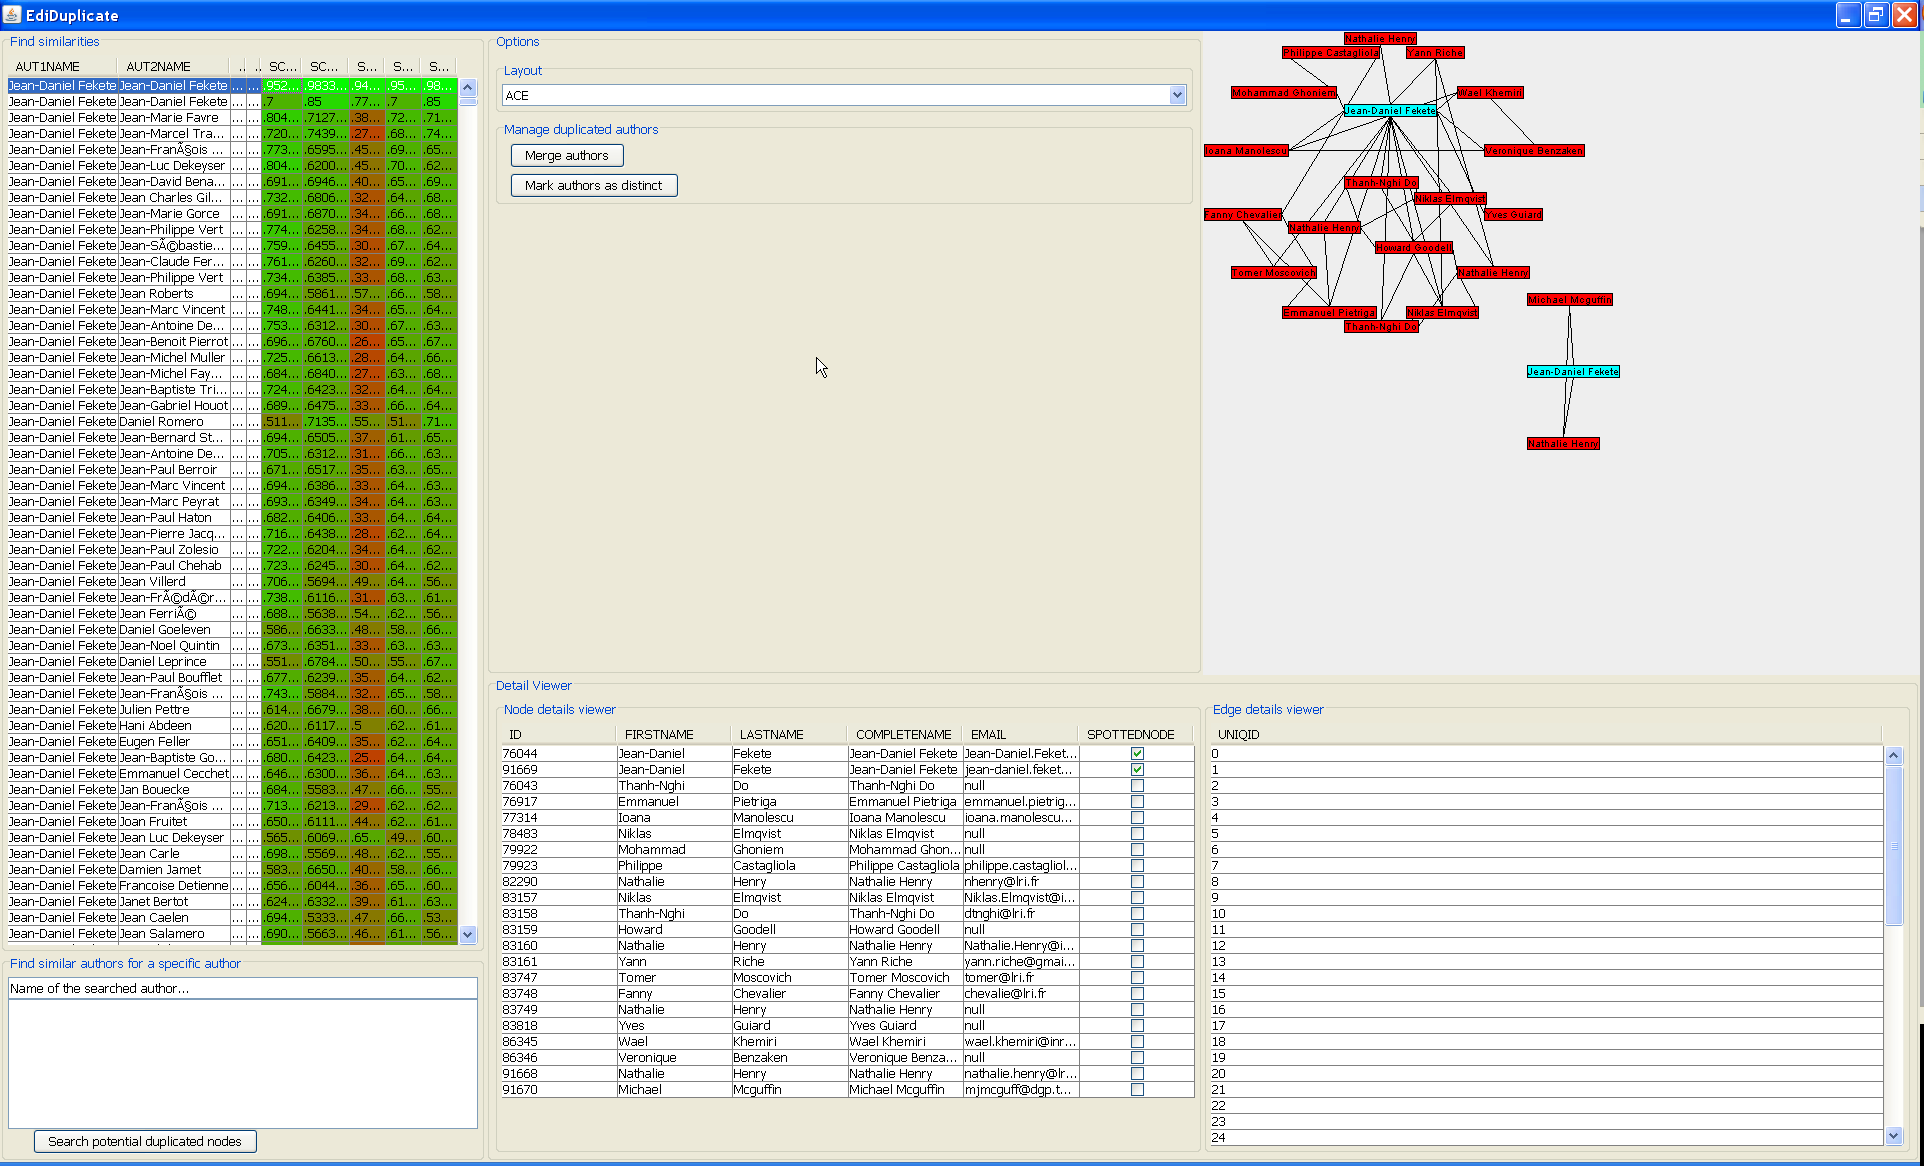
\includegraphics[width=\columnwidth]{figures/ediduplicate}
\caption{A screenshot of Ediduplicate}
\label{fig:ediduplicate}
\end{figure}

Our application EdiDuplicate offers the same possibilities but with extensions to cover specific needs. Concretely, we have implemented a loader to create an Obvious network from the  database. This structure is then fed by an external application with metrics for each pair of authors. Then, those statistics are displayed in a JTable (automically created from the Obvious structure). When, the user clicks on a cell a view of the neighbourhood of the current nodes is created. Then, with this information, the user is able to decide if the potential duplicated authors has to be merged. In addition, it is possible to query the Obvious structure to only display pair of duplicates for a specific authors. The user can also change the layout used to display the neighbourhood network with a JList: all graph layouts introduced in Infovis Toolkit are available. 

Concretely, the application mainly combines Obvious components and Swing components (derived from Obvious structure). For the data model, an Obvious Network is used (from the obvious-ivtk implementation), the visualization and the view part are also provided by this implementation. Building this application takes about less than a week.

\subsection{Implementing a cross-toolkit layout component}

Some of us have tested a potentially important usage scenario: devising a novel layout algorithm and using the Ovious toolkit to make it available in a variety of toolkits. This layout component is a generalized treemap algorithm.
% ~\cite{Treemaps2011}. 
Its interface makes it easy to port as this algorithm takes as input a data model and renders using a Visitor design pattern accross a renderer, making it very convenient to implement accross polyglyphic toolkits like prefuse or Discovery. Considering the current visualization model is mostly targeted at enabling monoglyphic patterns, Obvious in its current state turns out to be of limited use for our purpose.

Still, we have found that the existing data model and utilities have made developing our layout algorithm on top of Obvious worthwhile: we could implement very easily a simple monoglyphic visualization and view instances, and relying on the default data model already saves us time in the development of our prototype, while we have the assurance that only minimal work may be needed to port our method to the toolkits targeted by Obvious.


\section{Future work}


\subsection{Extending Obvious Supported Features}

Obvious aims at covering all the features of an information
visualization toolkit for which a consensual interface can be
specified.  Relying on a common reference model helps tremendously but
falls short on some implementation design choices.  Still, a few
specific services have already been mentioned during workshops that
could give rise to a shared implementation:

\begin{enumerate}
\item selection management: to implement cross-toolkit brushing and
  linking,
\item Mappings of data value to scalar value: this feature is used by
  all the visualizations to map data dimensions to screen coordinates,
  color gradients and many other visual attributes. Because the
  interface of such features is small and well understood, consensus
  is reachable,
\item visualization scale, tick-mark and tick-label management,
\item graph layout computation.
%\item ancillary panels, such as object editors.
\end{enumerate}

While most of those features would be of high value and we feel
consensus can be reached, we have not, as of yet, proposed unifying
designs.  The main reason is that while the core structure of those
services is consensual, they rely on parts which are not yet
consensual, such as the application architecture and more elaborated
view, visualization and interaction models.

\subsection{Adding Additional Toolkits and Languages}

\begin{comment}
% [jdf] I disagree. JViews is more like Piccolo or a structured
% graphics system. It is data-agnostic.  I am not sure how it would
% fit with Obvious.

A true test of how generalizable and unifying Obvious would be
post-hoc integration of a new toolkit. IBM ILOG JViews~\cite{JViews}
is one such example being considered. Because it is a commercial
product, this would have the advantage of bringing considerable
exposure to the platform.
\end{comment}

A wished extension would consist in porting the toolkit to other
languages and platforms, such as C++, JavaScript and C\#.  Obvious has
been designed to avoid using idioms too specific to Java so we believe
it could be done without much difficulties.  There would be at least
two benefits: the availability of a meta-toolkit is these languages to
wrap Information Visualization toolkits, and the availability of a
common application programmer's interface (API) for information
visualization that would simplify learning and spreading the best
practices.  Multi-language APIs already exist and are popular in
recommendations of the W3C. For example, the Document Object Model API
(DOM, see \url{http://www.w3.org/DOM/}) used to manipulate HTML or XML
documents has official bindings for Java and JavaScript and
non-standard bindings for several of the major languages
(\url{http://www.w3.org/DOM/Bindings}) with slight variations to cope
with the language idioms.

\begin{comment}
% C++ has generic containers in the STL (which is standard)
This
endeavor raises some new challenges: each language and platforms
supposes some specific idioms that are hardly translatable in concepts
of the other languages. Java has a generic collection type, for
instance, that does not map to a standard equivalent in C++. In
translating the design verbatim from a language to another, we would
insure some level of compatibility, but at the expense of
idiosyncrasies in our library, which would preclude widespread
adoption in our target languages. Conversely, adopting the target
language's idioms would preclude interoperability of the Obvious
platform across languages.
\end{comment}

\subsection{Community Building}

Perhaps the most novel experience we retain from Obvious is the
community-driven process to reach consensus and realize a reference
implementation.  We intend to formalize this process, either through a
formal consortium of with a less formal community-driven process,
depending on the response of the community.

\begin{comment}
 experiment on various means to carry this
community-driven consensus building, to see how it can help
consolidate acquired experience in the craft of toolkit design.


% thb style
In many respects, this process is akin to a
standardization process, only it lacks the industry incentive and
backing. Like open source projects, we shall only count on voluntary
contributions (aside partial of funding from public research grants),
only, in the present state of toolkits, it is much more tempting to
devise and expand one's own toolkit than contribute and make
compromise to use a shared design which still lacks serious adoption.


As an afterthought, we find such consolidation effort is rarely found
in research domains, and yet should surely help make the field more
visible and readable from an outsider perspective.
\end{comment}

\subsection{Obvious and Other Visualizations}

Visual Analytics often needs to combine Information Visualization with
Scientific Visualization and/or GeoSpatial Visualization.  These two
domains are more mature than information visualization for
standardization: the Scientific Visualization community is converging
towards using VTK~\cite{VTK} as a \textit{de facto} standard whereas
the GeoSpatial Visualization community already has a mature GeoSpatial
Consortium producing
software\footnote{\url{http://www.opengeospatial.org}}.

Geometrical data structures are much less sophisticated in information
visualization than in the two others visualization fields.
Pre-computing complex geometries and maintaining them dynamically is a
main concern in Scientific Visualization and GeoSpatial Visualization;
not so much in Information Visualization.  Moreover, even if at the
abstract level Scientific Visualization and GeoSpatial Visualization
share this concern, at the implementation level, their geometrical
structures are quite different, adding another level of complexity to
the problem.

Currently, the state of the art in combining these visualizations is
to put them side-by-side with coordinated interactions ( brushing and
linking, dynamic queries)~\cite{Coord3D}.  This kind of integration 
can be implemented by maintaining separate data structures, separate
visualizations and views; coordination being done through ad-hoc item
identifiers shared across the visualizations and acting as pivots.
From a user-centered viewpoint, unifying the interactions would also
improve the usability of mixed visualization applications.

Combining two or the three fields at the software infrastructure
level will require more discussions and experiments between the
communities and seems like a long-term goal.


\section{Conclusion}


We have presented Obvious, a meta-toolkit whose goal is, ultimately,
to consolidate the experience acquired by multiple toolkit designers
and contributors into a single tool. Obvious provides concrete,
immediate benefits to both toolkits designers and users: it dispenses
the former from re-implementing various mechanisms which are outside
their core concerns and helps them give visibility to their work by
integrating it into a global context. It enables the later (users) to
delay their choice of toolkit, be faced upfront with state of the art
design patterns as well as a wealth of convenience features. The
longer term benefits shall reach deeper prospects: possibly
defragmenting a research area by providing bridges between tools
rather than yet another, competing, toolkit. If this goal is
successfully reached, then the reward shall benefit the whole
information visualization community, enabling it to provide its user
communities an easier entry path. \emph{note from tb: it's getting
late, I'm not sure I can articulate my thoughts...}

Obvious shall remain a work in progress by design, at least in the
foreseeable future. All members of the visual analytics community are
invited to contribute to its design, make it evolve, and possibly use
its features. While Obvious may not yet be at a stage where it can be
diffused much beyond, this shall come soon. We hope it will prove a
valuable service to the visual analytics community.


%% if specified like this the section will be ommitted in review mode
\acknowledgements{
The authors wish to thank A, B, C. This work was supported in part by
a grant from XYZ.}

\bibliographystyle{abbrv}
%%use following if all content of bibtex file should be shown
\bibliography{obvious}
\end{document}
